% !Mode:: "TeX:UTF-8"
\title{实验六 MapReduce组件 实验报告}
\author{江昱峰 21009200038} 
\documentclass {article}
\usepackage[UTF8]{ctex}
\usepackage{graphicx}
\usepackage{float}
\usepackage{hyperref}
\usepackage{makecell}
\begin{document}
	%\begin{sloppypar}
	\maketitle{}
	\section{背景介绍}
		在学习JAVA知识时,我们知道JAVA的序列化框架(Serializable),它是JAVA本身自带的序列化框架,因为框架过于繁重,序列化对象包含很多额外信息(各种校验信息、header、继承体系等),不便于在网络之间进行高效传输。因此Hadoop开发了自己的序列化机制(Writable)
		
		在实际生产当中,假如有10亿条数据,我们通过MapReduce计算数据的最大值。在MapTask会产生大量的本地输出,如果不经过操作,直接由ReduceTask处理,将会在两者之间产生较大的网络IO,使得计算效率变慢,甚至程序崩溃。而使用Combiner可以减少在Map和Reduce节点之间的数据传输量,以提高网络IO性能,是MapReduce的一种优化手段之一。
	
	\section{实验目的}
		实践并掌握MapReduce组件,具体包括以下四部分内容:
		\begin{itemize}
			\item MapReduce序列化和排序;
			\item MapReduce分区;
			\item MapReduce的Combiner;
			\item MapReduce的自定义分组。
		\end{itemize}
	
	\section{实验知识}	
		\begin{itemize}
			\item 序列化概述:\\
			1. 序列化(Serialization):是指把结构化对象转化为字节流,以便于存储到磁盘(持久化)和网络传输。\\
			2. 反序列化(Deserialization):是序列化的逆过程。把字节流转为结构化对象。
			\item JAVA序列化:Java提供了一种对象序列化的机制,该机制中,一个对象可以被表示为一个字节序列,该字节序列包括该对象的数据、有关对象的类型的信息和存储在对象中数据的类型。将序列化对象写入文件之后,可以从文件中读取出来,并且对它进行反序列化,也就是说,对象的类型信息、对象的数据,还有对象中的数据类型可以用来在内存中新建对象。整个过程都是Java虚拟机(JVM)独立的,也就是说,在一个平台上序列化的对象可以在另一个完全不同的平台上反序列化该对象。类ObjectInputStream和ObjectOutputStream是高层次的数据流,它们包含反序列化和序列化对象的方法。
			\item MapReducec序列化:Hadoop中的序列化框架已经对基本类型和null提供了序列化的实现了。
			\item Combiner概论:Combiner是MR程序中Mapper和Reduce之外的一种组件,它的父类就是Reducer,Combiner和Reducer之间的区别在于运行位置,Reducer是每一个接收全局的MapTask所输出的结果,Combiner是在MapTask的节点中运行。简单理解为Combiner是局部聚合,是对每一个MapTask的输出进行汇总,减少数据在Map端和Reduce端的数据传输,提高运行效率的一种操作。而Reduce是全局的聚合操作。
		\end{itemize}
	
	\section{实验要求}
		掌握MapReduce组件,具体包括以下几个任务:
		\begin{itemize}
			\item 实现MapReduce序列化和反序列化。
			\item 通过自定义key(将数据封装为Bean对象作为key传输)实现排序功能。
			\item 通过自定义分区来完成相关需求的处理,得到最终的结果。
			\item 通过之前学习的WordCount案例,使用Combiner前后Reduce输入数据量大小进行对比。
			\item 计算给定的订单数据中每一个订单成交金额最大的一笔交易。
		\end{itemize}
	
	\section{实验环境}
		本次实验实验环境为青椒课堂平台的Linux(Centos 7.5)操作系统。
	
	\section{实验步骤}
		\subsection{MapReduce序列化和排序}
			\subsubsection{任务1:准备工作}
				数据准备:
				\begin{enumerate}
					\item 在/root/目录下创建sort.txt文件,内容如下:\\
					a	1 \\
					a	9 \\
					b	3 \\
					a	7 \\
					b	8 \\
					b	10 \\
					a	5
					
					\begin{figure}[H]
						\centering
						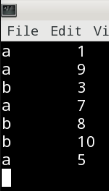
\includegraphics{figures/fig1.png}
					\end{figure}
				
					\item 字段解释:
					\begin{table}[H]
						\centering
						\begin{tabular}{|c|c|c|}
							\hline
							字段中文释义 & 字段英文释义 & 数据类型 \\ \hline
							字母 & word & String \\
							数字 & num & int \\ 
							\hline
						\end{tabular}
					\end{table}
				\end{enumerate}
			
				任务需求:
				\begin{enumerate}
					\item 实现MapReduce序列化和反序列化。
					\item 通过自定义key(将数据封装为Bean对象作为key传输)实现排序功能。
					\begin{itemize}
						\item 对第一列按字典进行排序。
						\item 第一列相同时对第二列按升序排列。
					\end{itemize}
				\end{enumerate}
	
				需求分析:要实现序列化和反序列化,通过实现Writable接口便可实现。但是又要完成对key的排序,需要通过实现WritableComparable中的compareTo方法来实现排序。
				
			\subsubsection{任务2:SortBean实现}
				该类主要用来将数据封装Bean对象,对数据进行序列化,反序列化和排序。
			
				程序步骤:
				\begin{enumerate}
					\item 实现WritableComparable接口。
					\item 定义字母和数字变量。
					\item 获取空参构造。
					\item 获取get和set方法。
					\item 重写序列化方法。
					\item 重写反序列化方法。
					\item 重写排序方法。
					\begin{itemize}
						\item 第一列按字典排序。
						\item 第一列相同时第二列升序排列。
					\end{itemize}
					\item 重写toString方法。
					\begin{figure}[H]
						\centering
						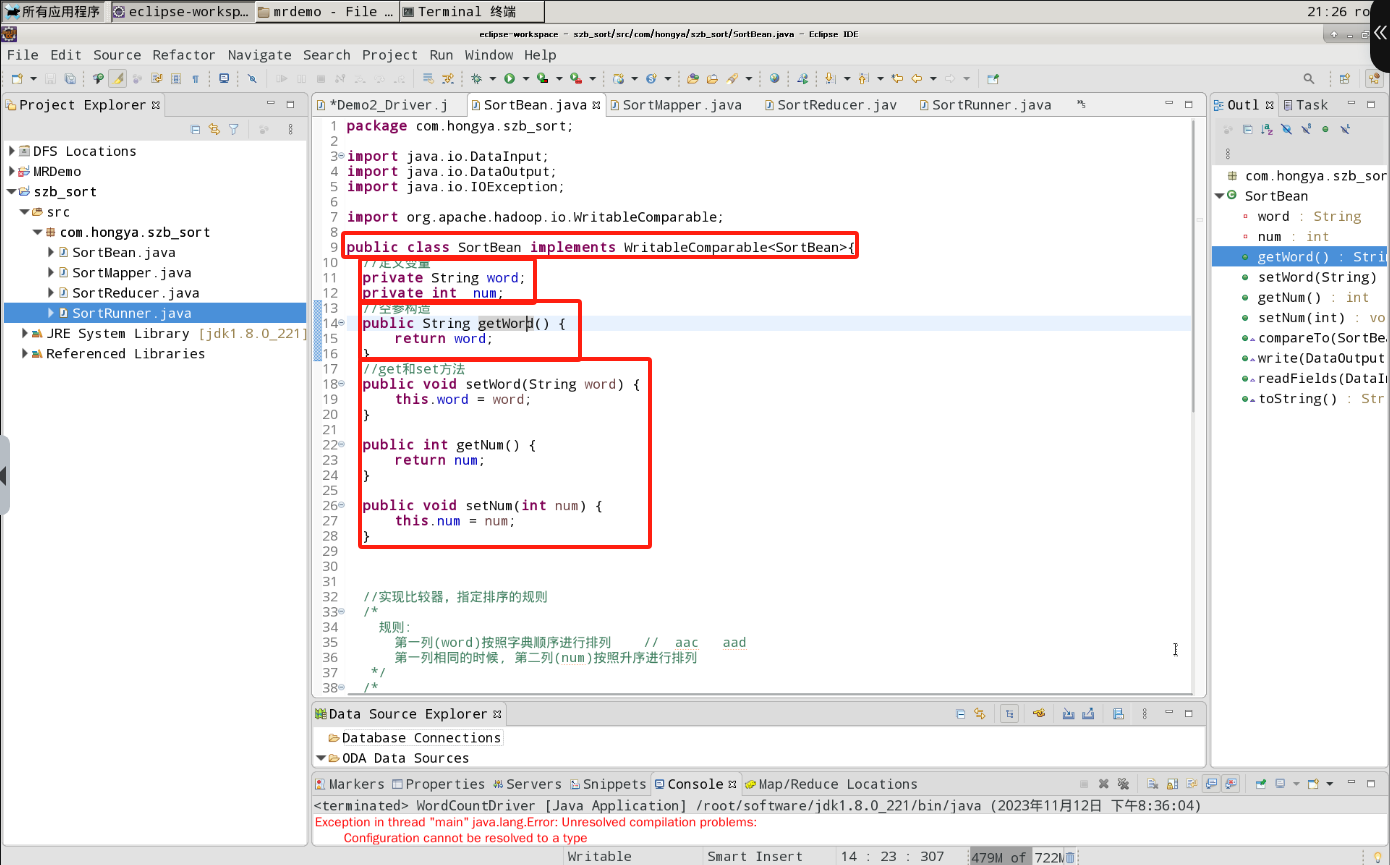
\includegraphics[width=4.5in]{figures/fig2.png}
					\end{figure}
					\begin{figure}[H]
						\centering
						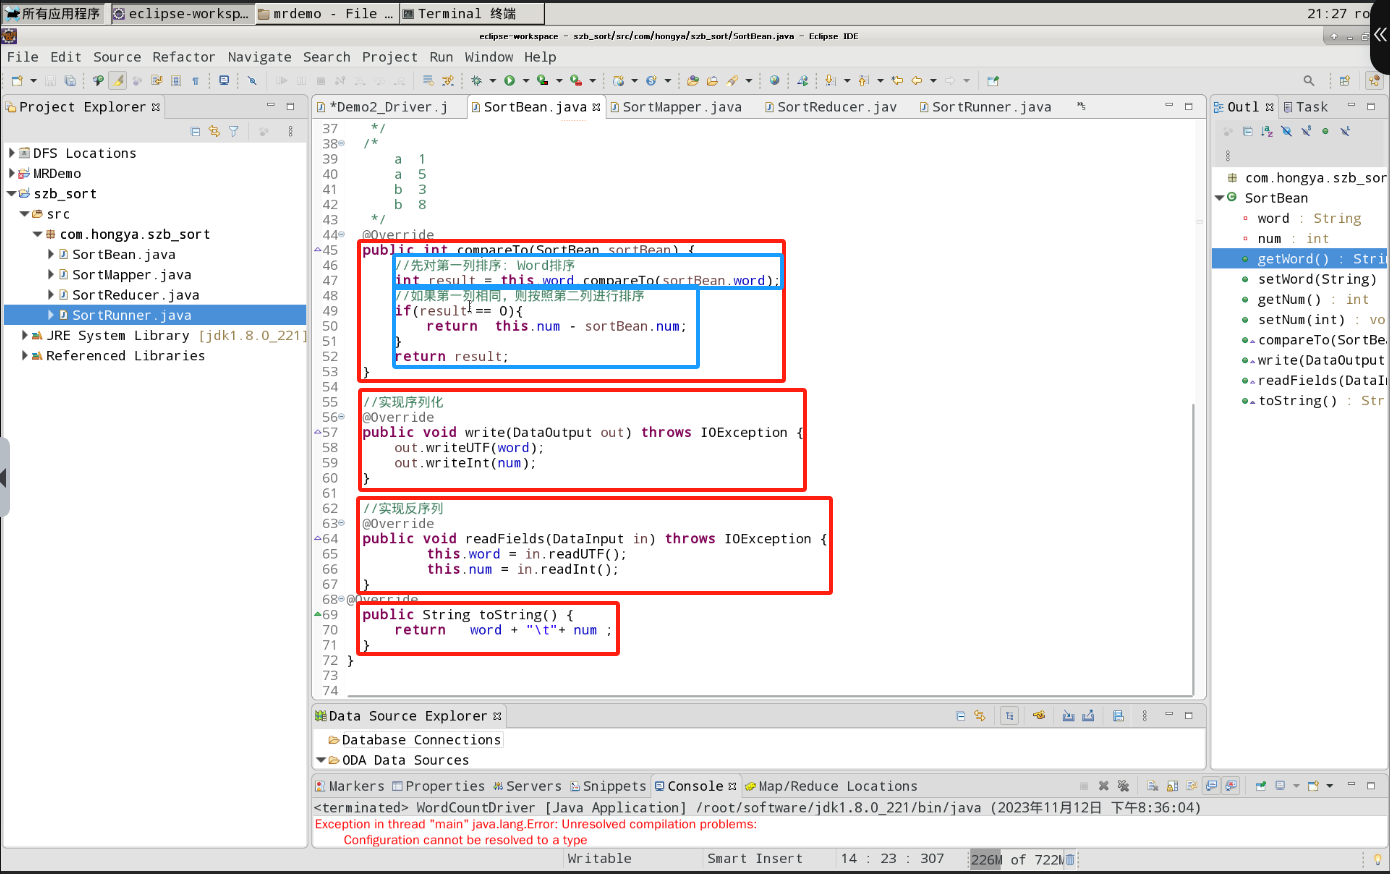
\includegraphics[width=4.5in]{figures/fig3.png}
					\end{figure}
				\end{enumerate}
			
			\subsubsection{任务3:SortMapper实现}
				Map端主要将文本数据进行转换,按需求将数据作为key,value记为空进行传输。
				
				程序步骤:
				\begin{enumerate}
					\item 继承Mapper。
					\item 重写map方法,将数据按\textbackslash{}t进行切割。
					\item 将数据收集到SortBean对象。
					\item 将SortBean作为key,value记为空。
					\begin{figure}[H]
						\centering
						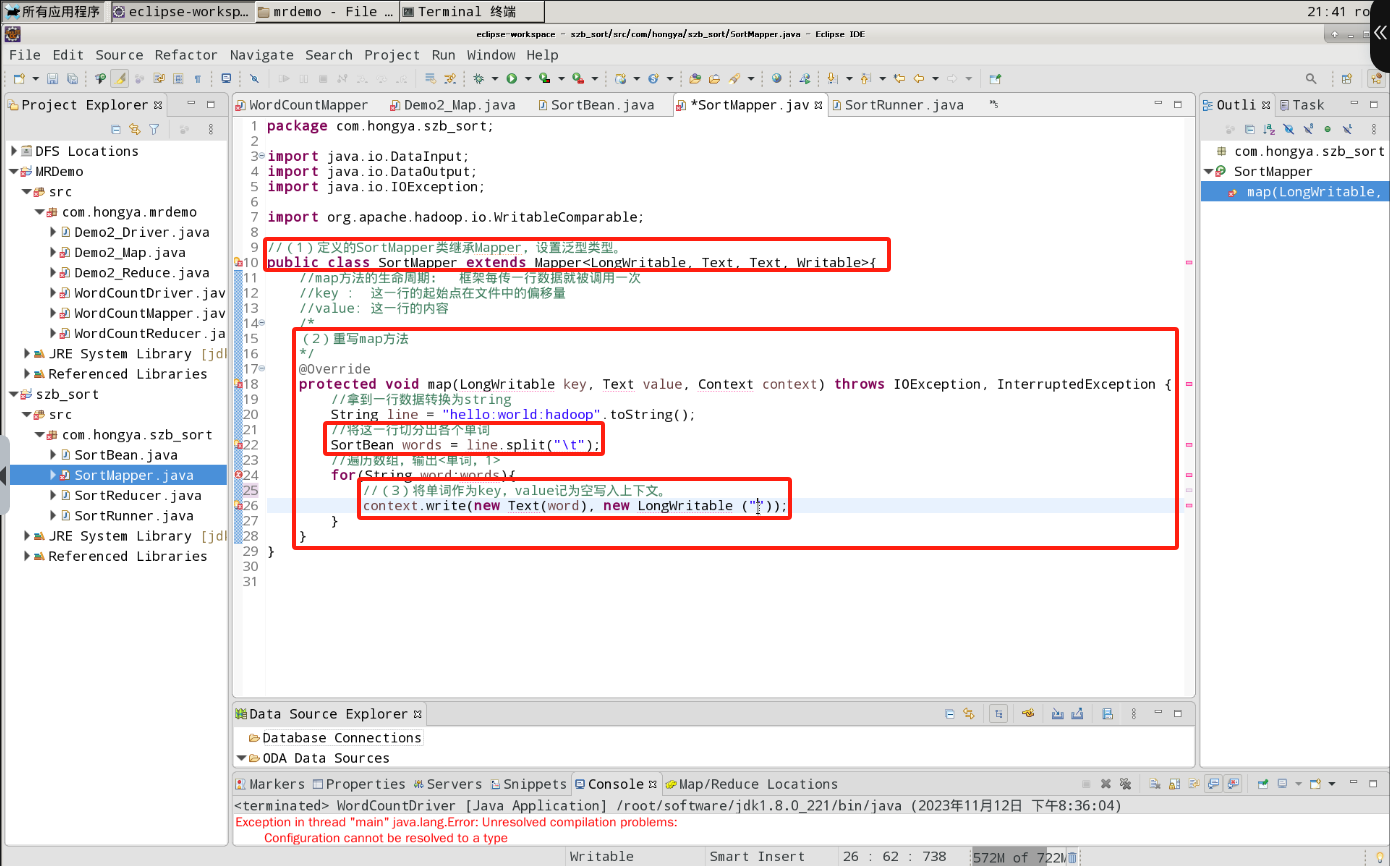
\includegraphics[width=4.5in]{figures/fig4.png}
					\end{figure}
				\end{enumerate}
				
			\subsubsection{任务4:SortReducer实现}
				Reduce端主要将K2和V2转为K3和V3,不需要其他操作,因此可直接对数据进行收集。
				
				程序步骤:
				\begin{enumerate}
					\item 继承Reducer类。
					\item 重写reduce方法。
					\item 收集数据。
					\begin{figure}[H]
						\centering
						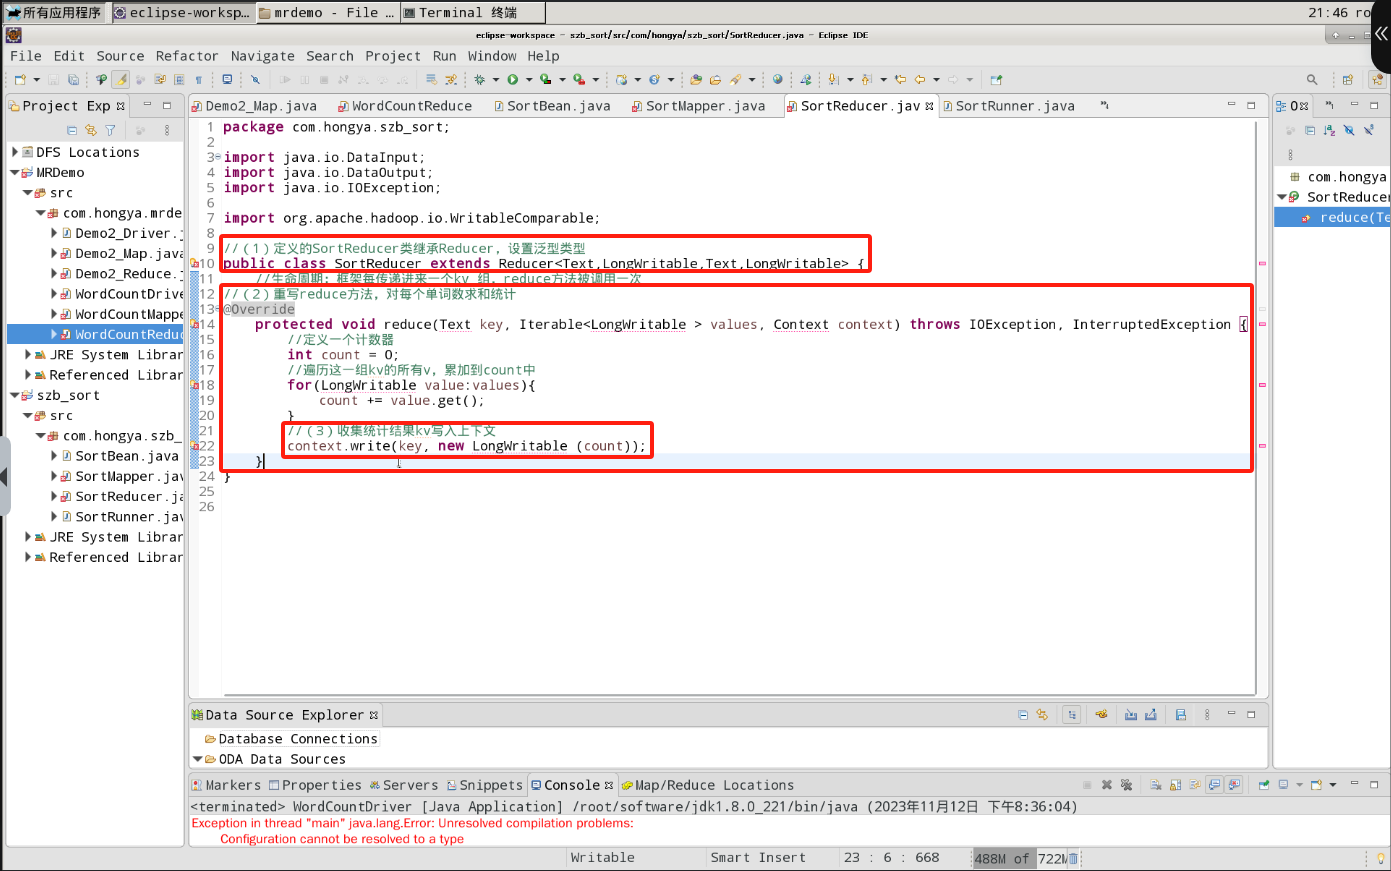
\includegraphics[width=4.5in]{figures/fig5.png}
					\end{figure}
				\end{enumerate}
			
			\subsubsection{任务5:SortRunner实现}
				程序主入口(SortRunner)程序步骤:
				\begin{enumerate}
					\item 创建建一个job任务对象。
					\item 指定job所在的jar包。
					\item 指定源文件的读取方式类和源文件的读取路径类:/root/sort.txt。
					\item 指定自定义的Mapper类和K2、V2类型。
					\item 指定自定义的Reducer类和K3、V3的数据类型。
					\item 指定输出方式类和结果输出路径:/root/output/。
					\item 将job提交到yarn集群。
					\begin{figure}[H]
						\centering
						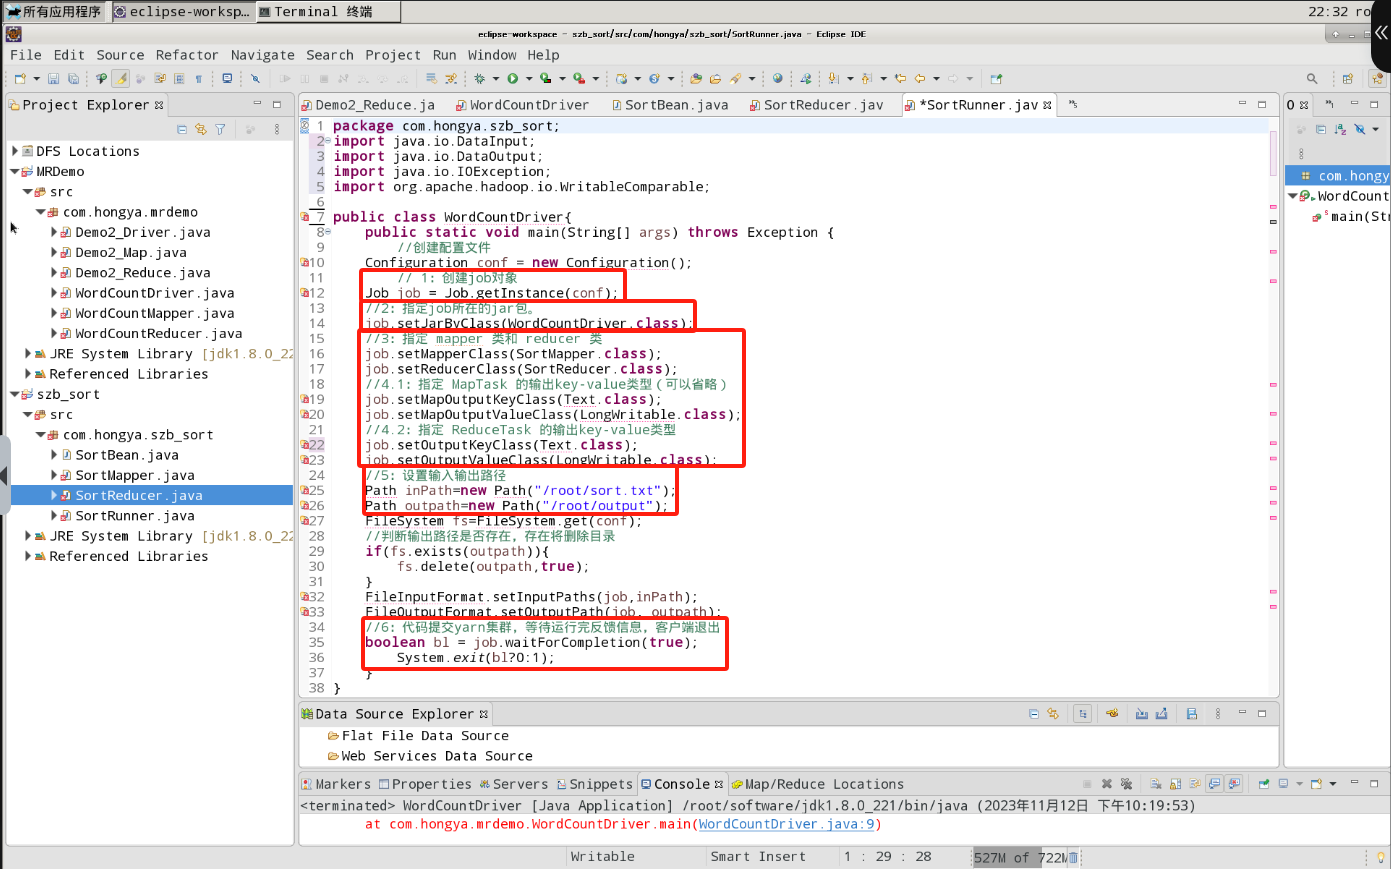
\includegraphics[width=4.5in]{figures/fig6.png}
					\end{figure}
				\end{enumerate}
			
				运行程序。
				
				使用cat命令查看结果。
				\begin{figure}[H]
					\centering
					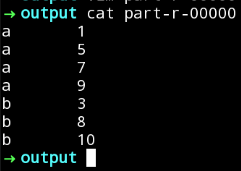
\includegraphics{figures/fig7.png}
				\end{figure}
			
		\subsection{MapReduce分区}
			任务:MapReduce分区案例实现
			
			主要针对自定义分区进行操作,在Map端和Reduce端只进行传递操作,不做任何逻辑处理。
			\subsubsection{数据样例:}
				partition.csv文件如下所示,数据为某彩票开奖数据,其中第五个字段表示开奖结果数值,本节实训我们只对第五列数据进行研究分析。
				
				"1	0	1	2017-07-31 23:10:12	837255	6	4+1+1=6	小","双	0	0.00	0.00	1	0.00	1	1" \\
				"2	0	1	2017-07-31 23:15:03	837256	14	4+7+3=14	大","双	0	0.00	0.00	1	0.00	4	1" \\ 
				"3	0	1	2017-07-31 23:20:12	837257	17	6+9+2=17	大","单	0	0.00	0.00	1	0.00	3	1" \\
				"4	0	1	2017-07-31 23:25:12	837258	22	5+8+9=22	大","双	0	0.00	0.00	1	0.00	2	1" \\
				"5	0	1	2017-07-31 23:30:18	837259	1	1+0+0=1	小","单	0	0.00	0.00	1	0.00	2	1" \\
				"6	0	2	2017-07-31 23:17:22	2170779	4	2+0+2=4	小","双	0	0.00	0.00	1	0.00	2	1" \\
				"7	0	2	2017-07-31 23:20:49	2170780	12	1+2+9=12	小","双	0	0.00	0.00	1	0.00	1	1" \\
				"8	0	2	2017-07-31 23:24:18	2170781	11	6+4+1=11	小","单	0	0.00	0.00	1	0.00	3	1" \\
				"9	0	2	2017-07-31 23:27:43	2170782	20	5+7+8=20	大","双	0	0.00	0.00	1	0.00	3	1" \\
				"10	0	2	2017-07-31 23:31:23	2170783	12	3+1+8=12	小","双	0	0.00	0.00	1	0.00	1	1" \\
				"11	0	2	2017-07-31 23:34:52	2170784	11	3+1+7=11	小","单	0	0.00	0.00	1	0.00	3	1" \\
				"12	0	1	2017-07-31 23:35:09	837260	20	8+7+5=20	大","双	0	0.00	0.00	1	0.00	3	1" \\
				"13	0	2	2017-07-31 23:38:20	2170785	23	5+9+9=23	大","单	0	0.00	0.00	1	0.00	3	1" \\
				"14	0	1	2017-07-31 23:40:19	837261	13	3+2+8=13	小","单	0	0.00	0.00	1	0.00	4	1" \\
				"15	0	2	2017-07-31 23:41:56	2170786	15	3+8+4=15	大","单	0	0.00	0.00	1	0.00	1	1" \\
				"16	0	1	2017-07-31 23:45:09	837262	14	2+5+7=14	大","双	0	0.00	0.00	1	0.00	4	1" \\
				"17	0	2	2017-07-31 23:45:24	2170787	7	4+3+0=7	小","单	0	0.00	0.00	1	0.00	2	1" \\
				"18	0	2	2017-07-31 23:48:51	2170788	14	4+3+7=14	大","双	0	0.00	0.00	1	0.00	4	1" \\
				...
				
				\begin{figure}[H]
					\centering
					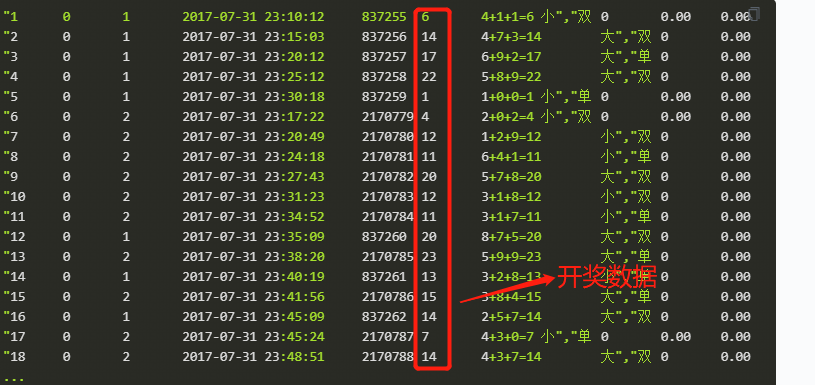
\includegraphics[width=4.5in]{figures/fig8.jpg}
				\end{figure}
		
			\subsubsection{案例需求}
				将第五列数据中15以上的结果以及15以下的结果进行分开成两个文件进行保存。
			
			\subsubsection{准备工作}
				\begin{enumerate}
					\item 点击上传按钮上传partition.csv数据,上传路径为/root/partition.csv。
					\item 创建MapReduce项目:
					\begin{itemize}
						\item 项目名:partition。
						\item 包结构:com.hongya.partition。
						\item Map端实现类:MyMapper。
						\item 自定义Partition类:MyPartition。
						\item Reduce端实现类:MyReducer。
						\item 主程序实现类:PartitionRunner。
						\begin{figure}[H]
							\centering
							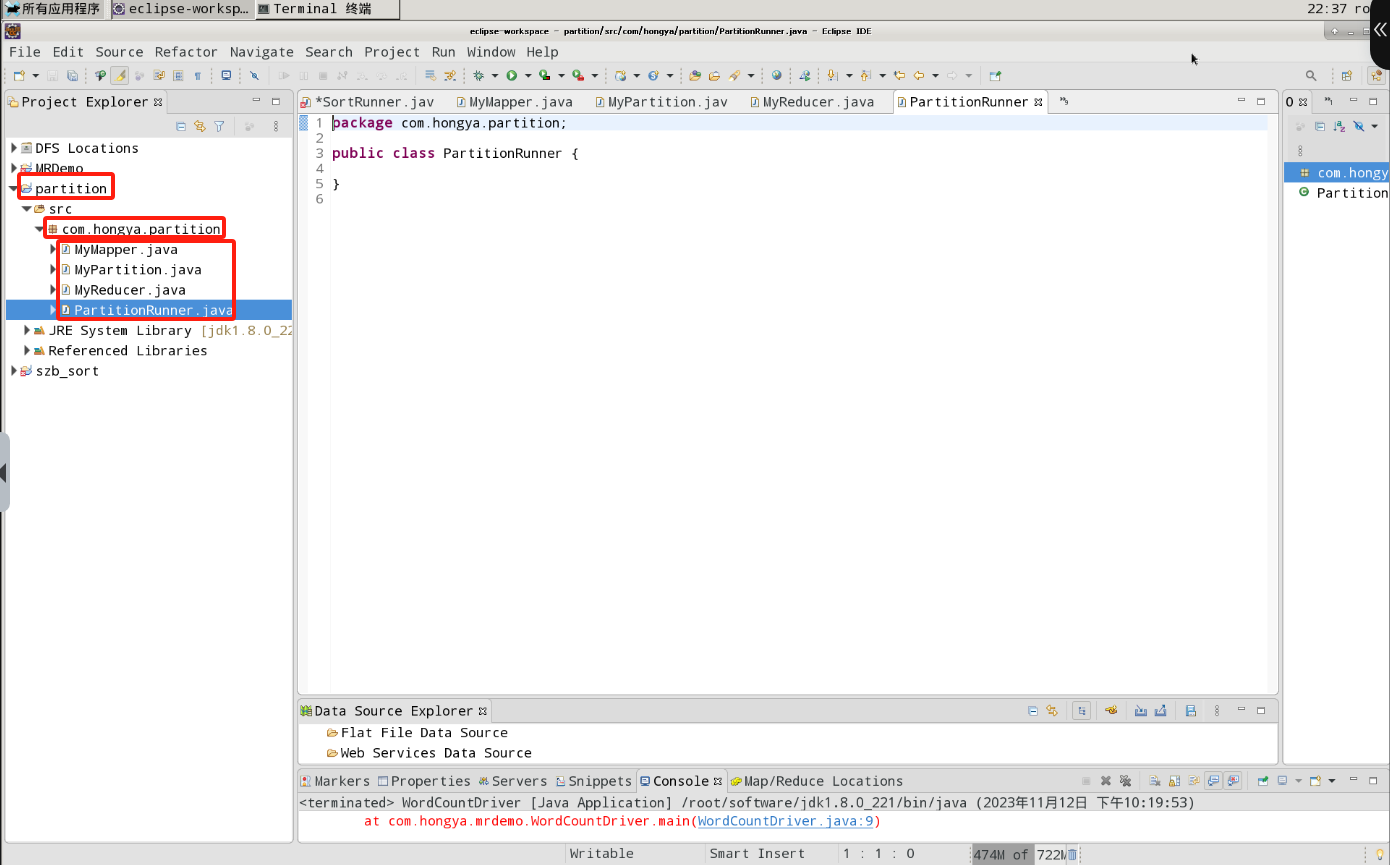
\includegraphics[width=4.5in]{figures/fig9.png}
						\end{figure}
					\end{itemize}
				\end{enumerate}
				
			\subsubsection{程序实现}
				\begin{enumerate}
					\item Map端程序不做任何逻辑, 也不对Key-Value做任何改变, 只是接收数据, 然后往下发送。
					\begin{figure}[H]
						\centering
						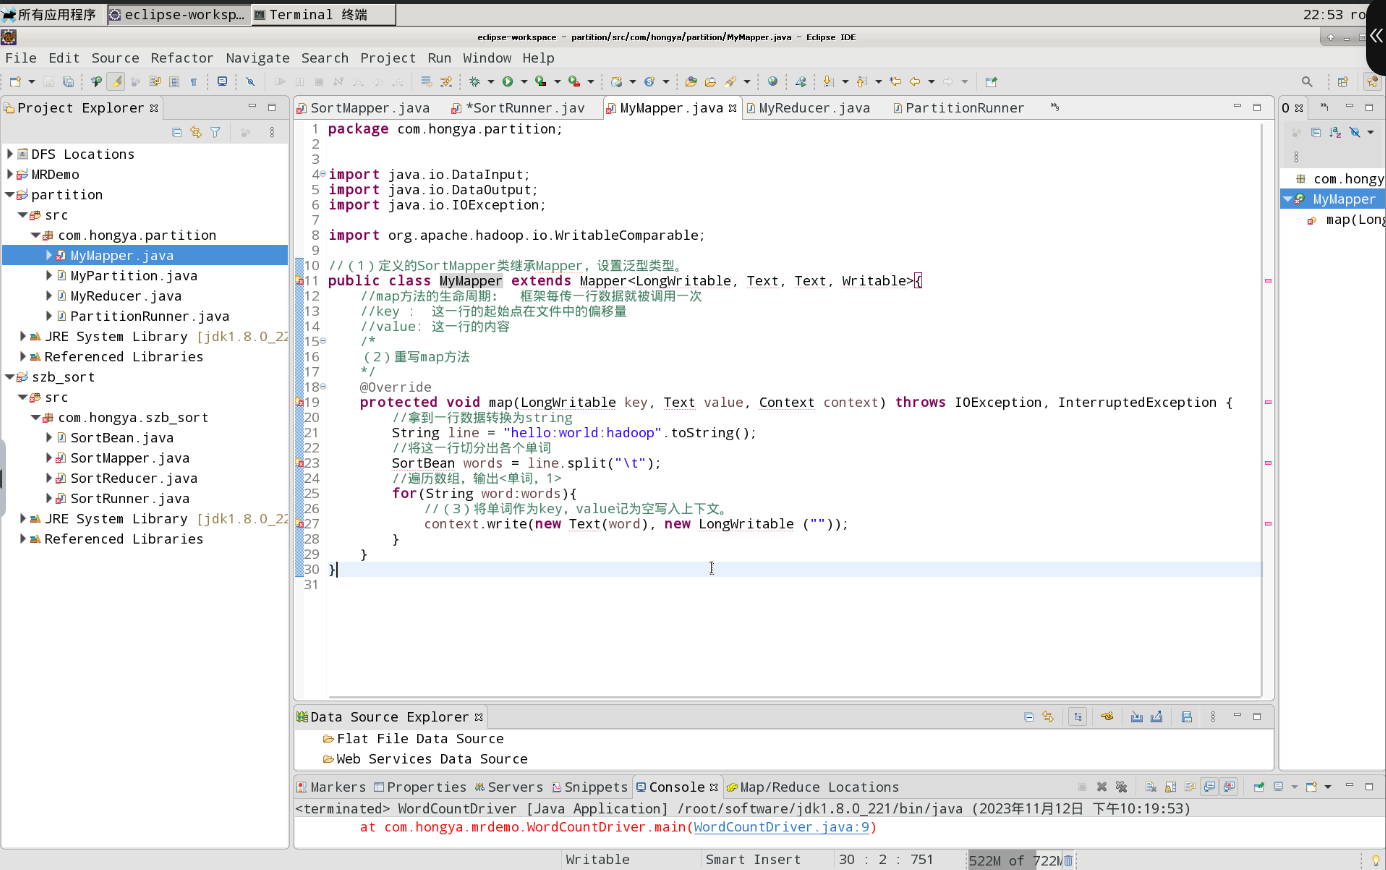
\includegraphics[width=4.5in]{figures/fig10.png}
					\end{figure}
				
					\item Reduce端也不做任何处理, 将数据原封不动输出即可。
					\begin{figure}[H]
						\centering
						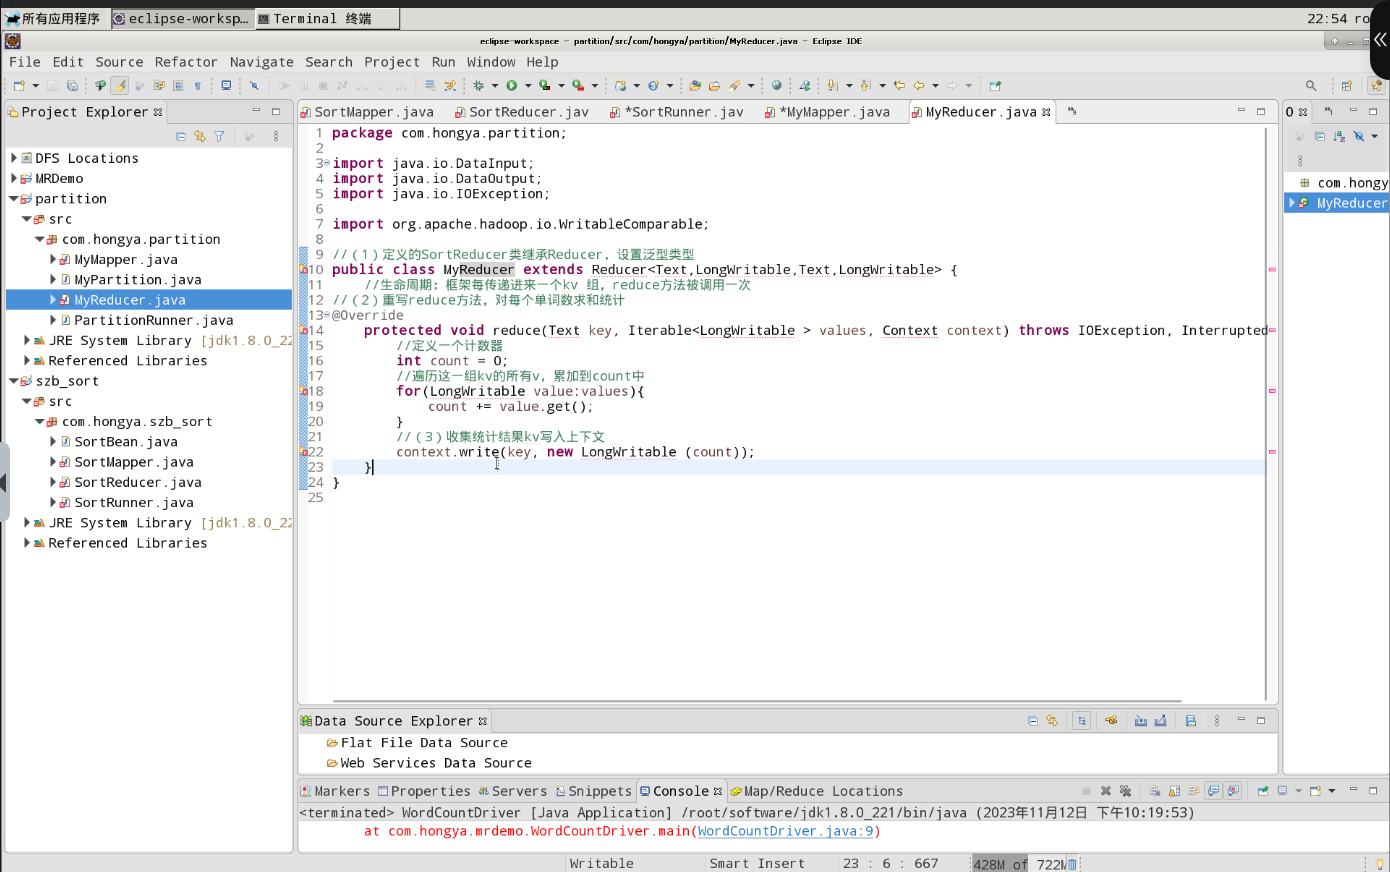
\includegraphics[width=4.5in]{figures/fig11.png}
					\end{figure}
				
					\item 自定义Partitioner类实现。
					\begin{itemize}
						\item 继承Partitioner类。
						\item 重写getPartition()方法。
						\item 获取数据切分出第五列开奖结果数值数据。
						\item 大于十五的分区返回1,否则返回0。
						\begin{figure}[H]
							\centering
							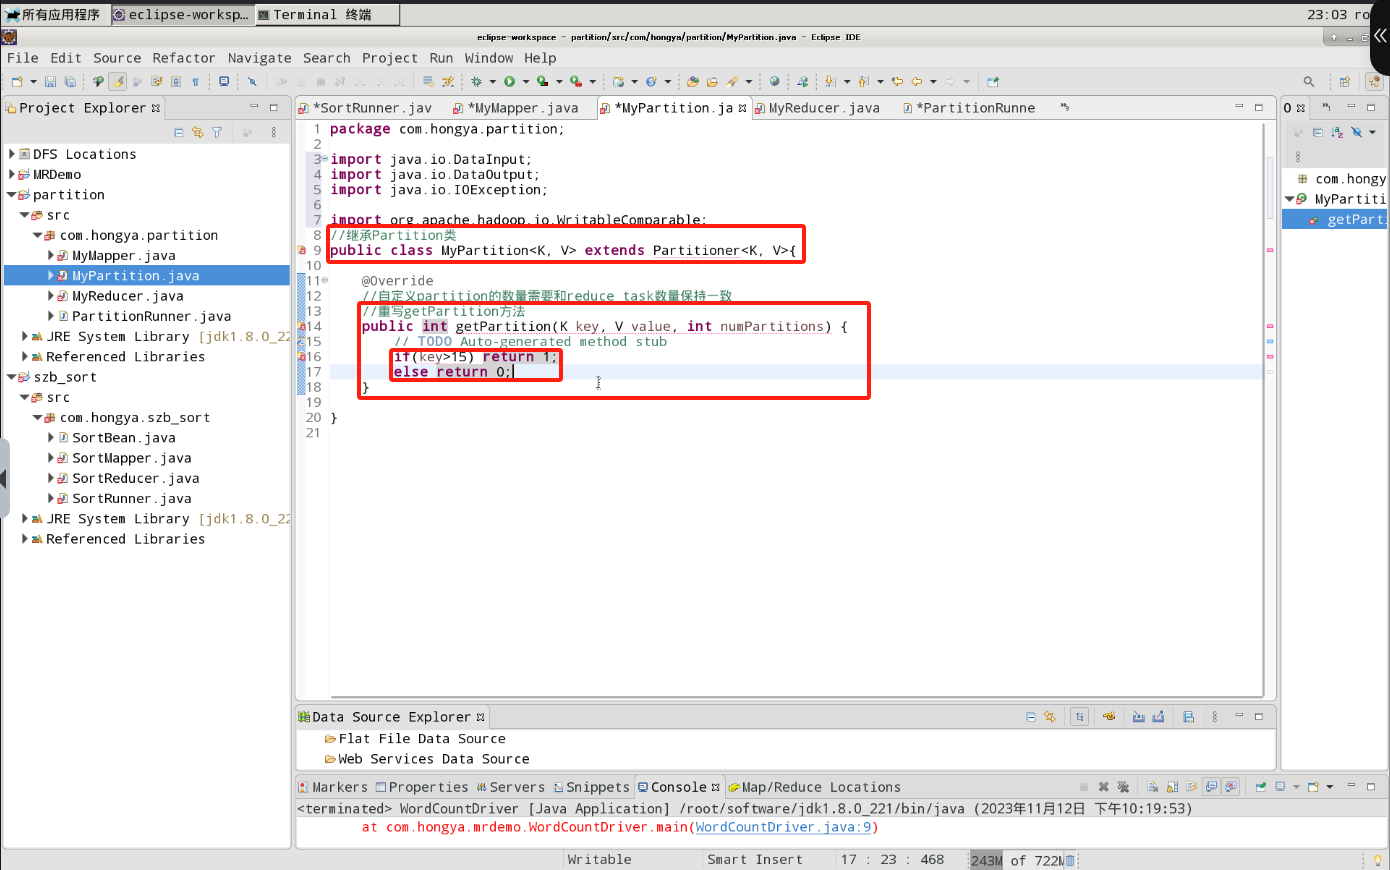
\includegraphics[width=4.5in]{figures/fig12.png}
						\end{figure}
					\end{itemize}
				
					\item 主程序类PartitionRunner实现:
					\begin{itemize}
						\item 创建job任务对象。
						\item 指定job所在的jar包。
						\item 指定源文件的读取方式类和源文件的读取路径。
						\item 指定自定义的Mapper类和k2、v2类型。
						\item 指定分区类。
						\item 指定自定义的Reducer类和k3、v3的数据类型。
						\item 设置ReduceTask的个数和分区数相同。
						\item 指定输出方式类和结果输出路径。
						\item 将job提交给yarn集群。
						\begin{figure}[H]
							\centering
							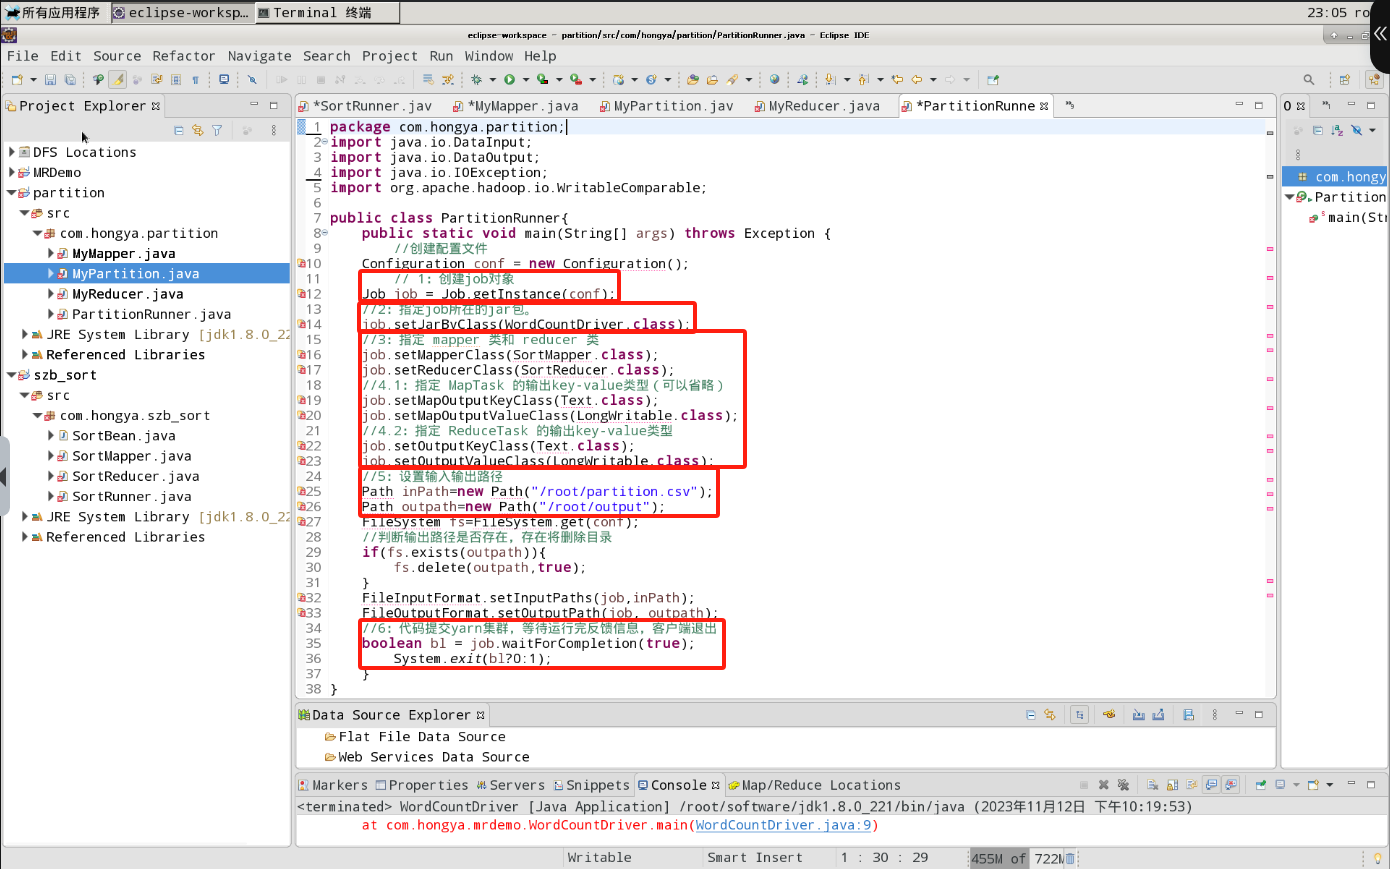
\includegraphics[width=4.5in]{figures/fig13.png}
						\end{figure}
					\end{itemize}
				\end{enumerate}
				
			\subsubsection{查看结果文件}
				根据需求要求,我将文件分成了两个。因此程序最终运行成功后会在输出路径下生成两个文件part-r-00000和part-r-00001,通过cat命令查看两个文件即可。
				
		\subsection{MapReduce的Combiner}
			任务:Combiner演示
				\begin{enumerate}
					\item 准备工作
					\begin{enumerate}
						\item WordCount案例代码所在路径为:/root/practice/hadoopcode/com/hongya/combiner/WordCount.java。
						\item 数据所在路径为:/root/practice/hadoopdata/combiner.txt。
						\item MapReduce项目创建:
						\begin{itemize}
							\item 项目名:combiner
							\item 包结构:com.hongya.combiner。
							\item Combiner实现类:MyCombiner。
						\end{itemize}
						\begin{figure}[H]
							\centering
							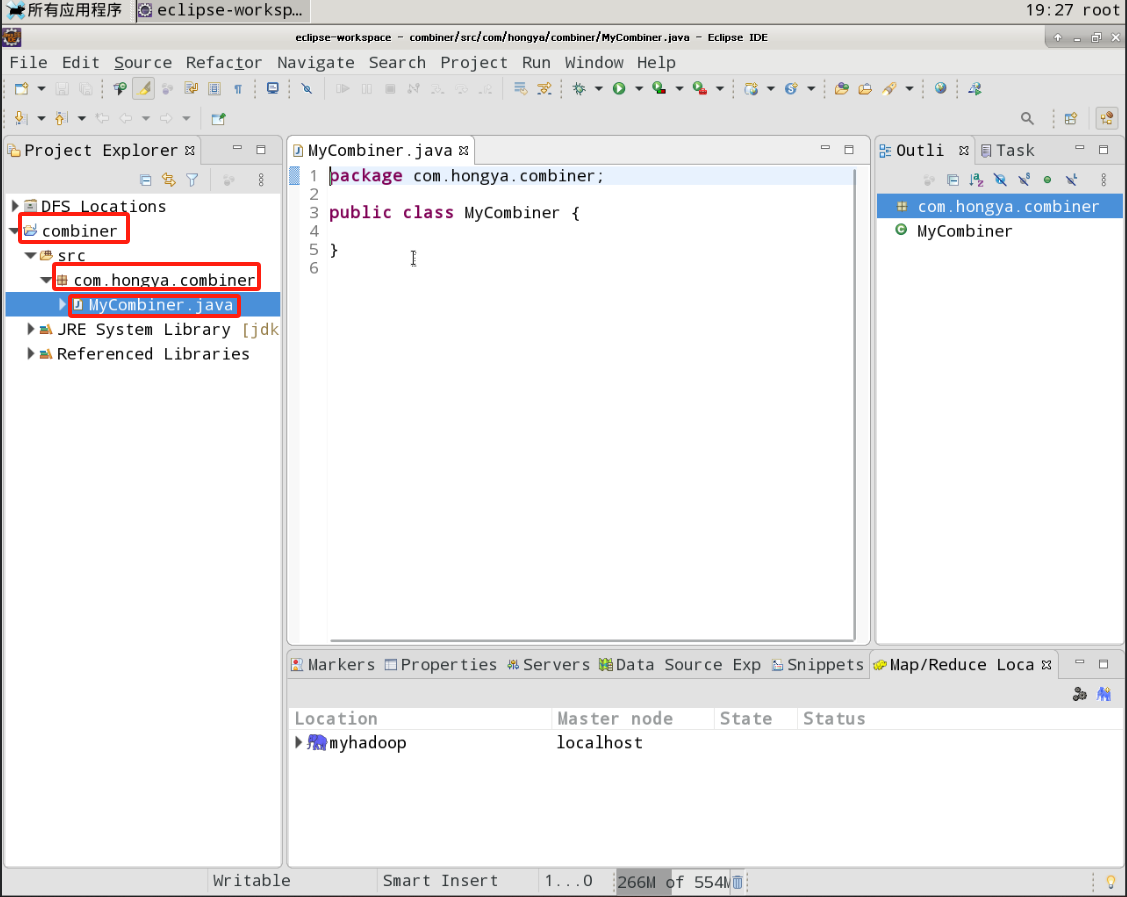
\includegraphics[width=4.5in]{figures/fig15.jpg}
						\end{figure}
					
						\item 将WordCount案例代码拷贝到创建的项目目录下。
					\end{enumerate}
				
					\item 运行程序,查看日志中Reduce输入数据量。
					\item 实现Combiner代码逻辑:
						\begin{itemize}
							\item MyCombiner类继承Reducer类。
							\item 重写reduce方法。
							\item 定义累加变量count。
							\item 遍历集合,进行累加求和操作。
							\item 将单词作为key,count值作为value进行收集。
						\end{itemize}
					\begin{figure}[H]
						\centering
						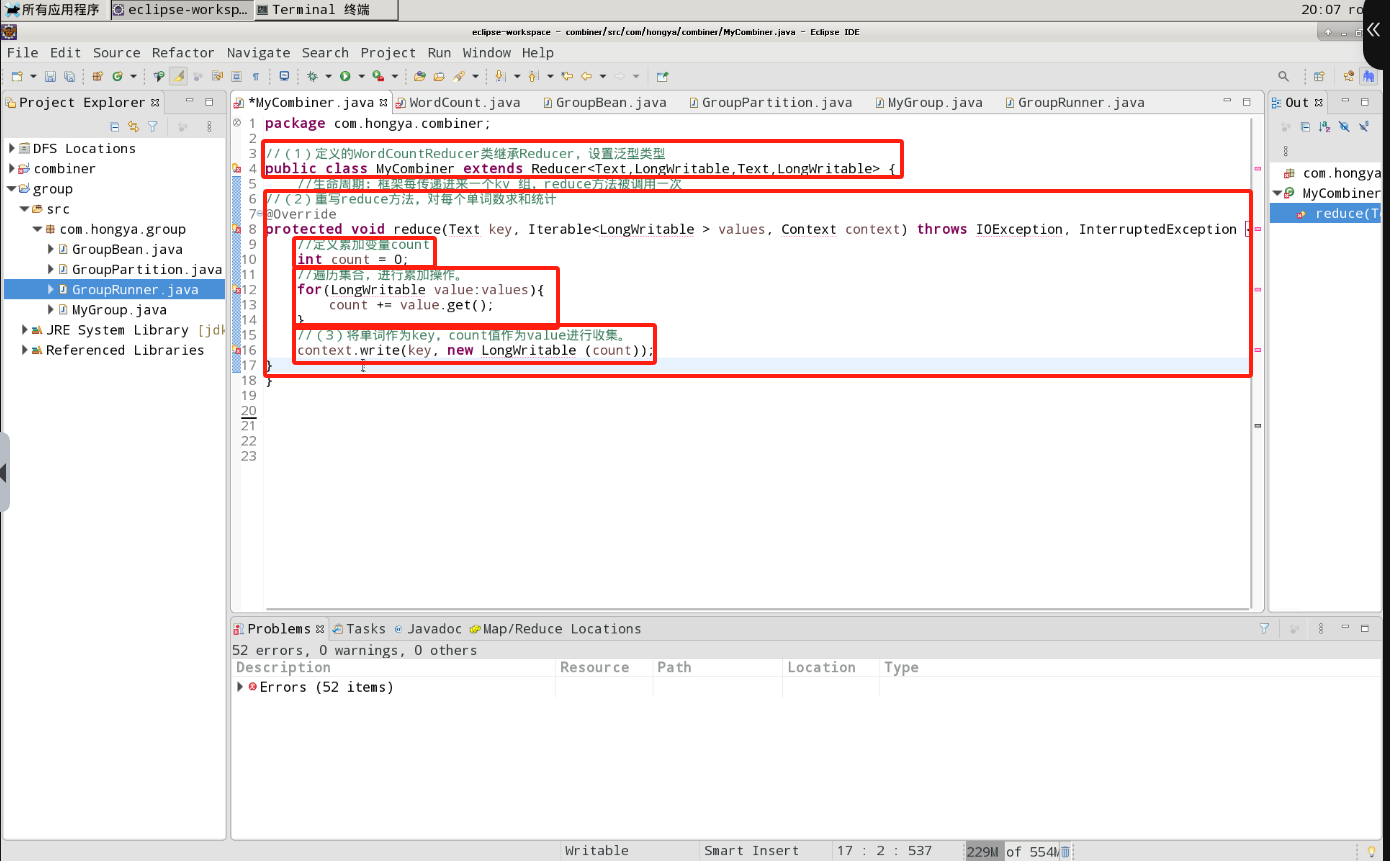
\includegraphics[width=4.5in]{figures/fig17.jpg}
					\end{figure}
				
					\item 在主程序中添加Combiner类。
					\item 运行程序,查看日志中Reduce输入数据量。
					\item 比较使用Combiner前后Reduce输入数据量是否相同。
				\end{enumerate}
			
		\subsection{MapReduce的自定义分组}
			\subsubsection{任务1:GroupBean类实现}
				在分组实现中我们知道必须要注册数据对象类,因此我们需要将数据进行封装,根据需求可知,我们需要将订单id,金额进行封装。

				上传数据:点击按钮上传group.txt文件,文件上传路径为:/root/。
					
				MapReduce项目创建:
				\begin{enumerate}
					\item 项目名:group。
					\item 包名:com.hongya.group。
					\item 类:
					\begin{itemize}
						\item 封装数据对象类:GroupBean。
						\item 自定义分区类:GroupPartition。
						\item 自定义分组类:MyGroup。
						\item 主程序以及Map,Reduce端处理类:GroupRunner。
					\end{itemize}
				\end{enumerate}
				\begin{figure}[H]
					\centering
					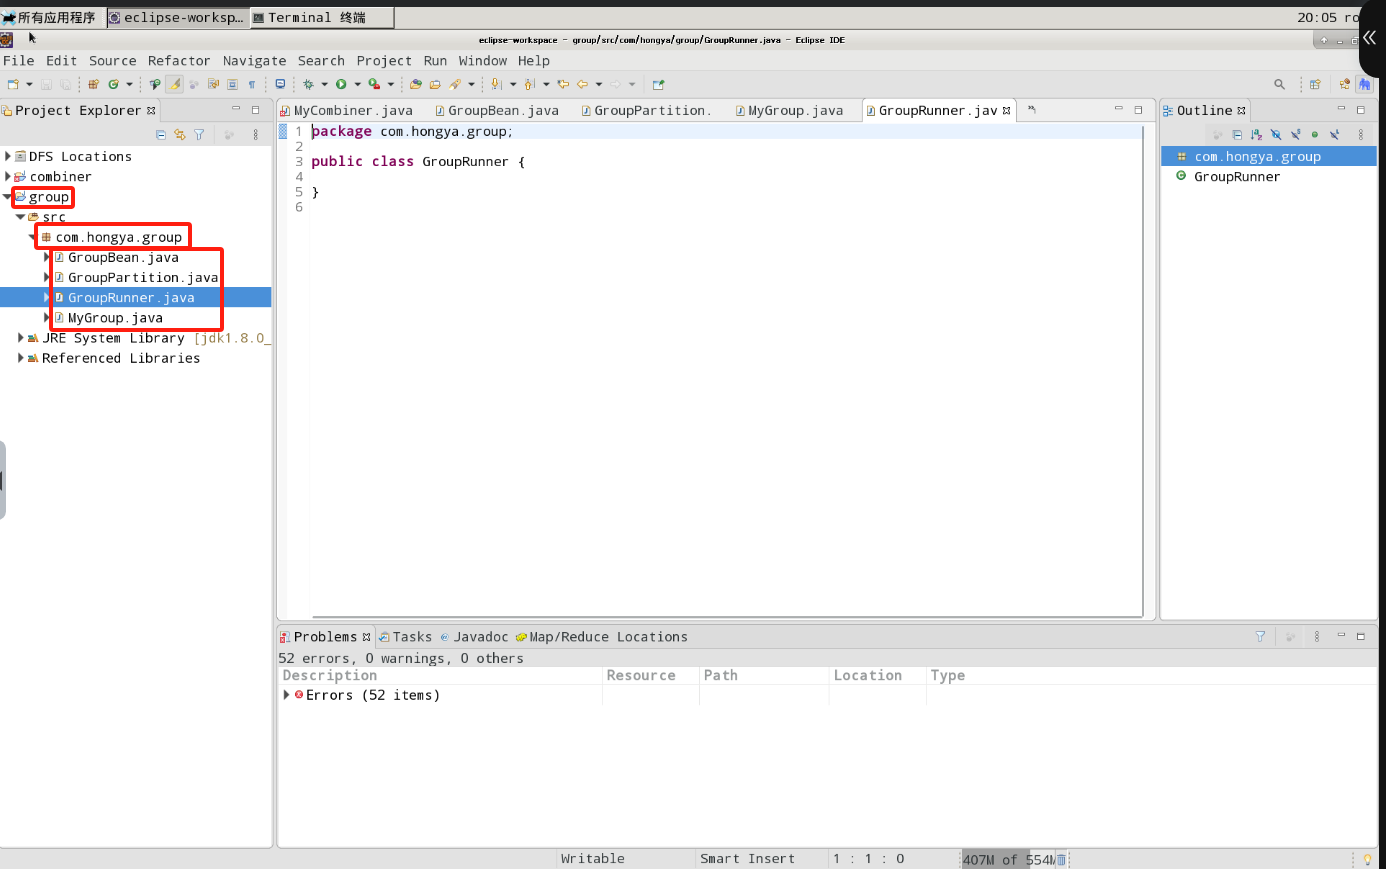
\includegraphics[width=4.5in]{figures/fig19.jpg}
				\end{figure}
			
				GroupBean实现逻辑:
				\begin{enumerate}
					\item GroupBean实现WritableComparable<>接口。
					\item 定义字段订单id,金额。
					\item 获取空参,全参构造。
					\item 获取get和set方法。
					\item 重写排序方法compare To()。
					\item 在排序中按订单id排序,订单Id相同按金额降序排列。
					\item 重写序列化和反序列化。
					\item 重写toString方法。	
				\end{enumerate}
				\begin{figure}[H]
					\centering
					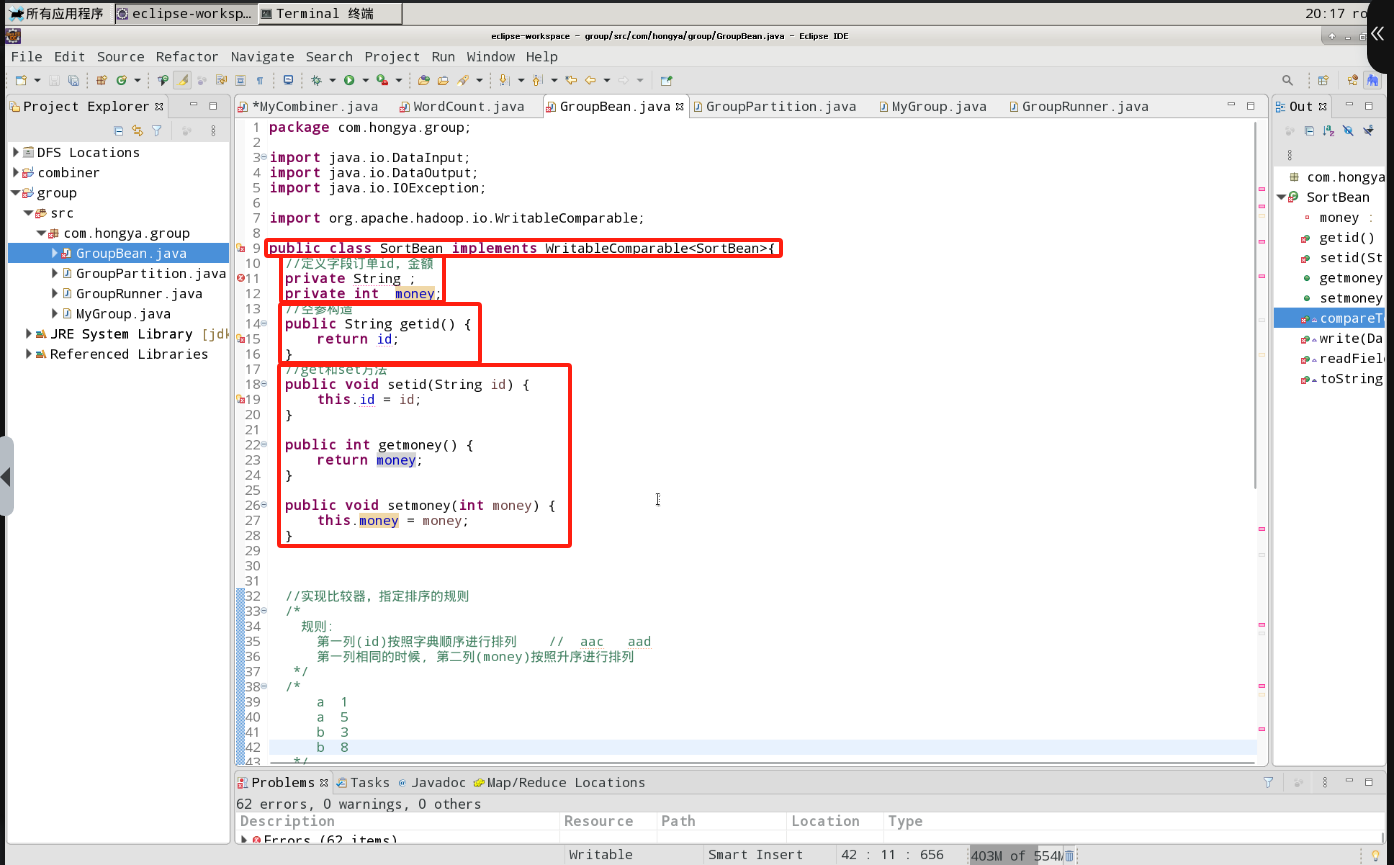
\includegraphics[width=4.5in]{figures/fig20.jpg}
				\end{figure}
				\begin{figure}[H]
					\centering
					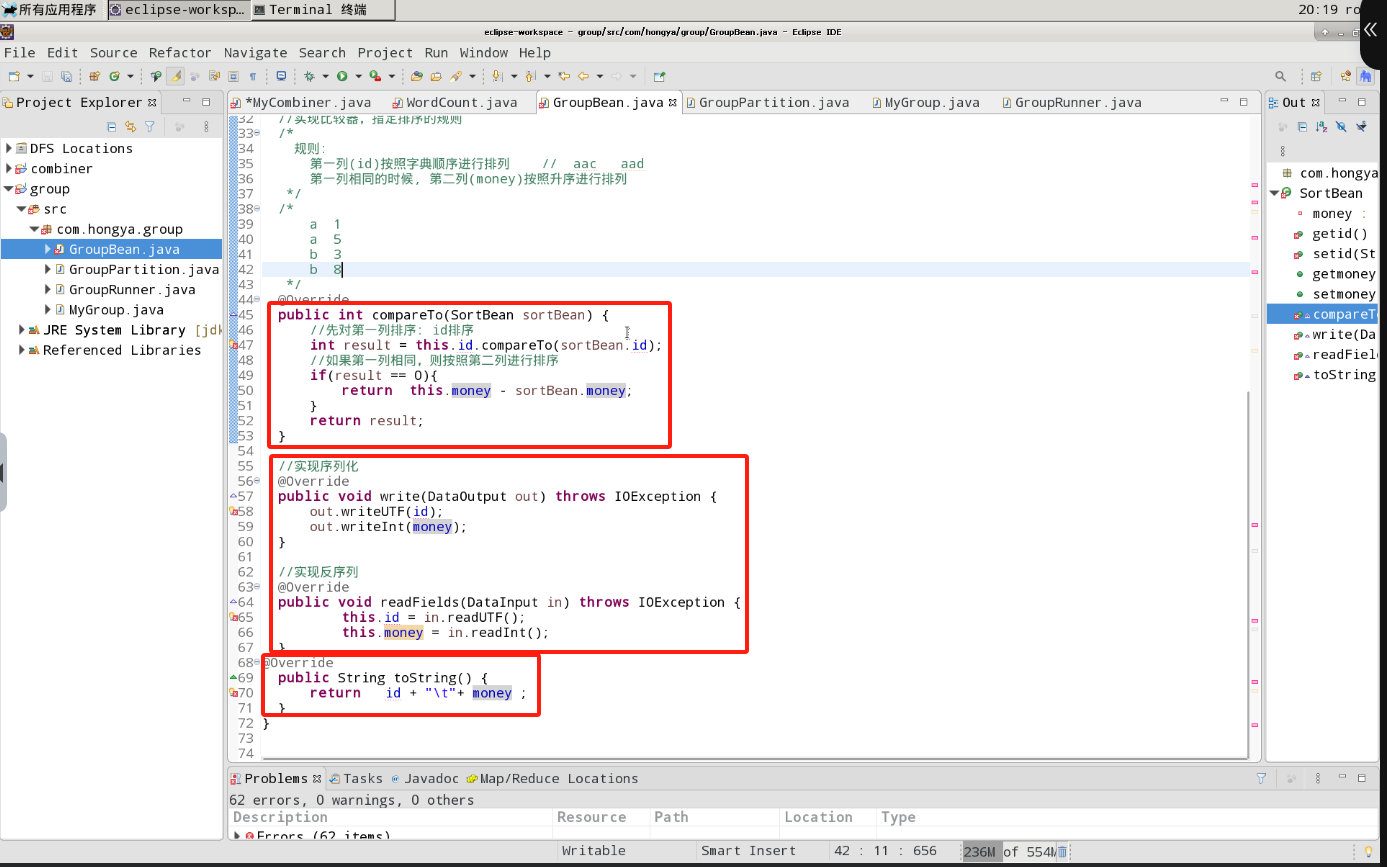
\includegraphics[width=4.5in]{figures/fig21.jpg}
				\end{figure}
				
			\subsubsection{任务2:分区分组实现}
				需要自定义分区分组,分区中按照订单id进行分区,把所有订单id相同的数据,都发送到同一个Reduce中去。分组中通过比较相同的订单id,将相同的放入同一个组,同一个组的已经排好序,直接TopN获取最大数据。
				
				分区逻辑实现:
				\begin{enumerate}
					\item GroupPartition继承Partition。
					\item 重写getPartition方法。
					\item 将相同订单id的数据发送到同一个Reduce中。
				\end{enumerate}
				\begin{figure}[H]
					\centering
					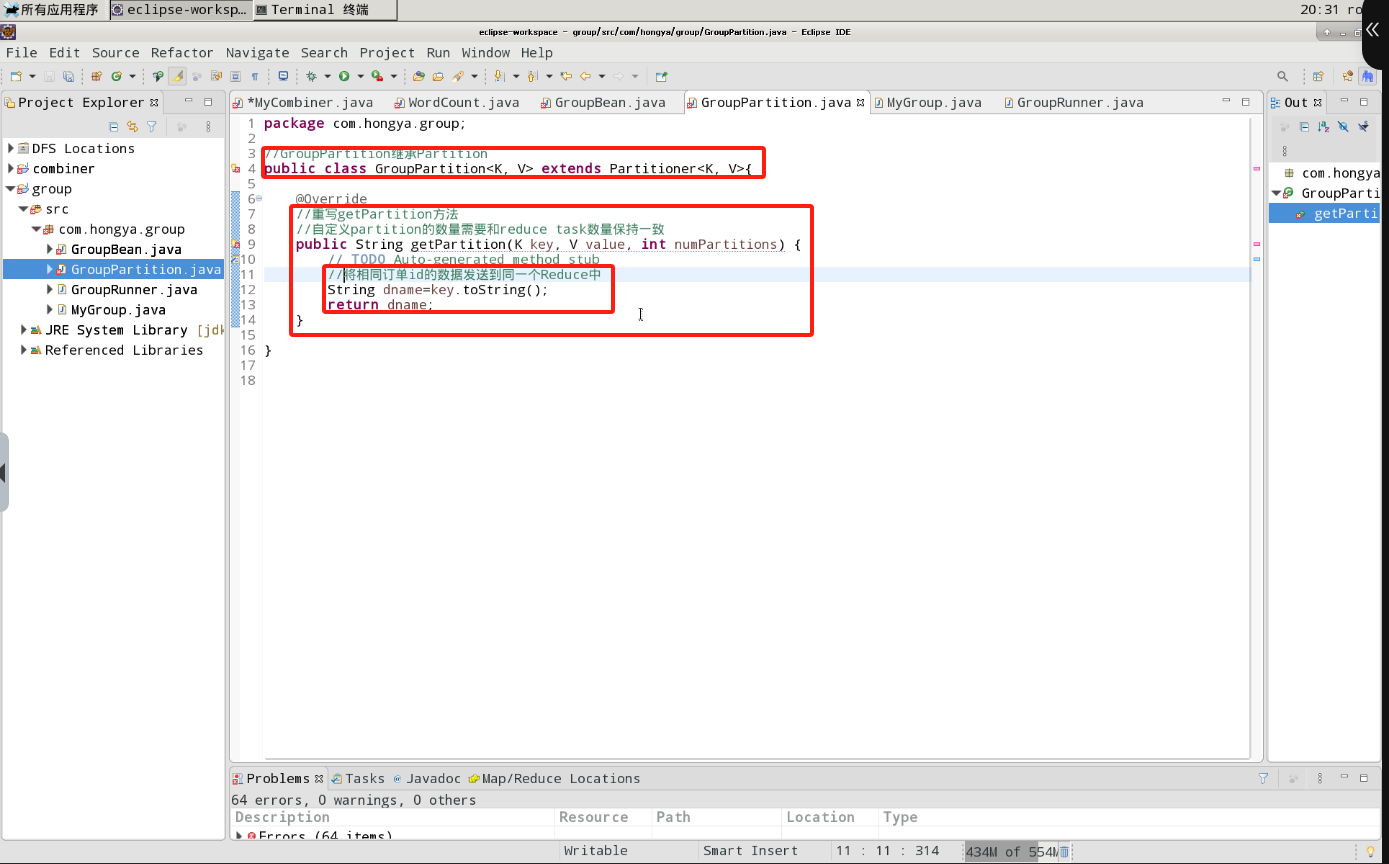
\includegraphics[width=3.5in]{figures/fig22.jpg}
				\end{figure}
			
				分组逻辑实现:
				\begin{enumerate}
					\item MyGroup继承WritableComparator类。
					\item 将定义的GroupBean注册到MyGroup中。
					\item 重写compare方法。
					\item 比较两个对象中的订单id是否是同一组并进行返回。
				\end{enumerate}
				\begin{figure}[H]
					\centering
					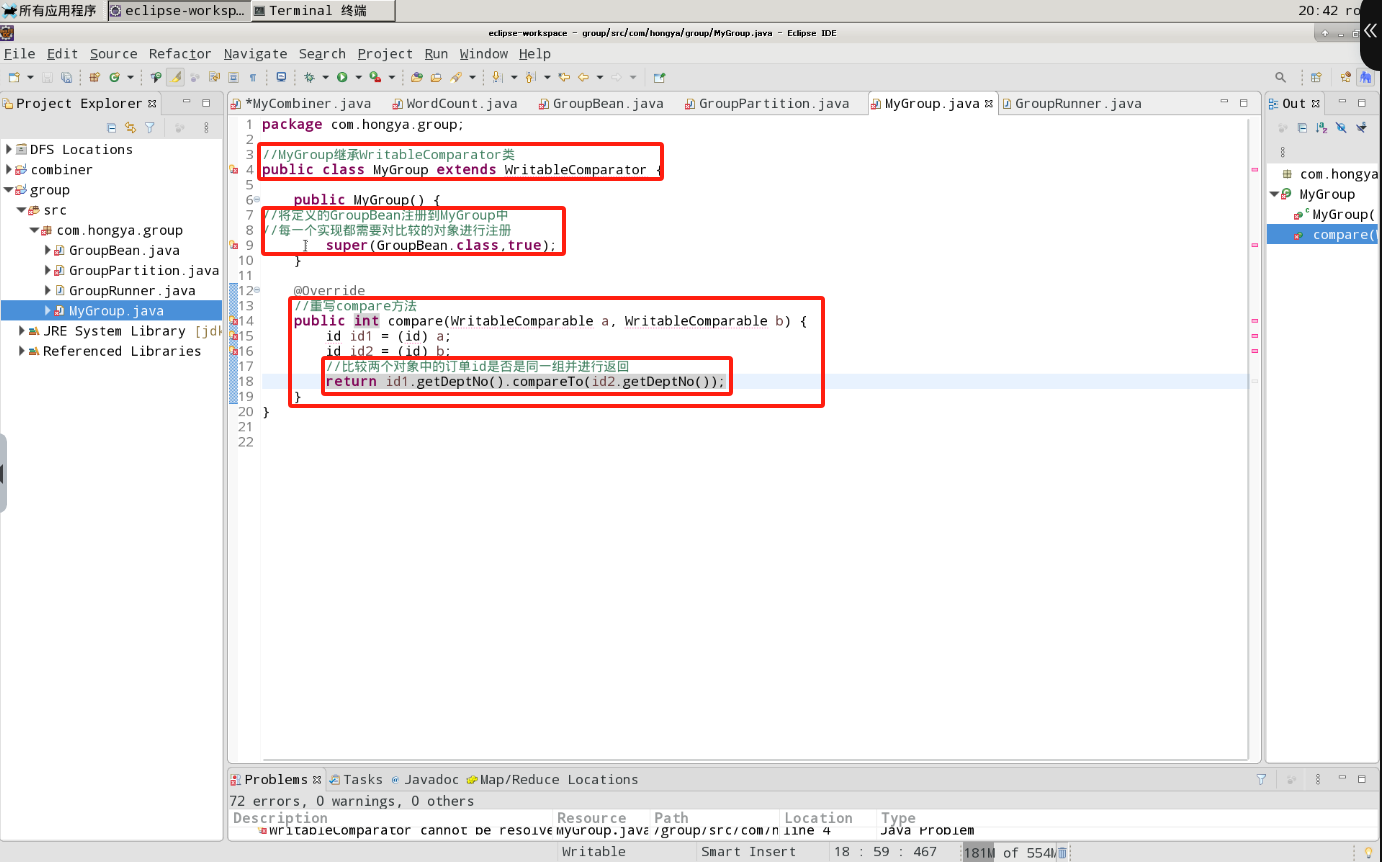
\includegraphics[width=3.5in]{figures/fig23.jpg}
				\end{figure}
					
			\subsubsection{任务3:主程序以及Map,Reduce端实现}
				将程序主入口以及Map,Reduce端逻辑整合到GroupRunner类中进行实现。
				
				程序主入口实现:
				\begin{enumerate}
					\item 在main方法中创建job对象。
					\item 指定job所在的jar包。
					\item 指定Mapper类为MyMaaper,Reducer类为MyReducer。
					\item 指定MapTask和ReduceTask的输出key-value类型。
					\item 设置分区类。
					\item 设置分组类。
					\item 设置ReduceTask数为3。
					\item 设置数据输入输出格式。
					\item 设置输入路径为/root/group.txt,输出路径为/root/output/。
					\item 将job提交给yarn集群。
				\end{enumerate}
				\begin{figure}[H]
					\centering
					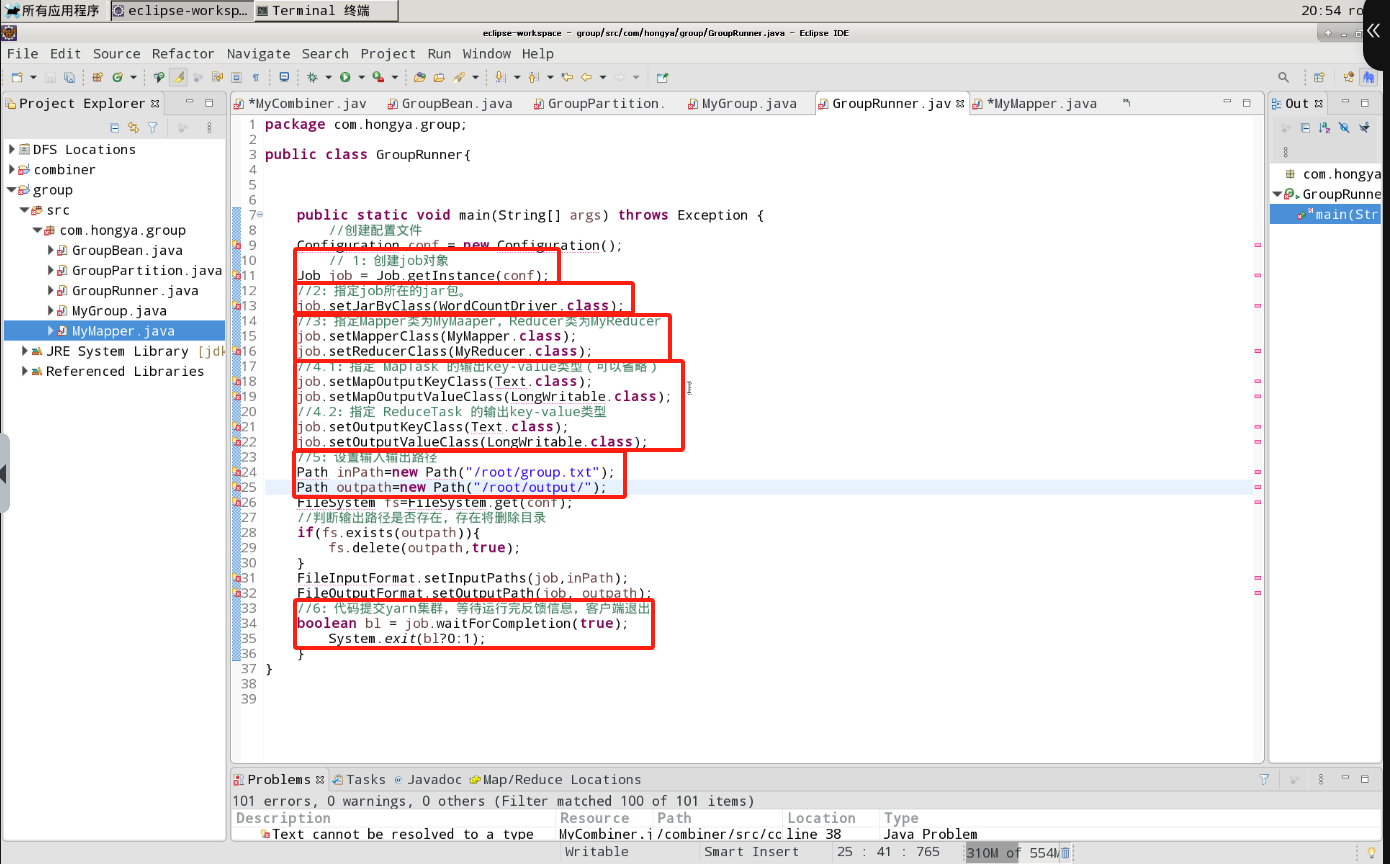
\includegraphics[width=4.5in]{figures/fig24.jpg}
				\end{figure}
			
				Map端实现:
				\begin{enumerate}
					\item 定义MyMapper类继承Mapper。
					\item 重写map方法。
					\item 获取每行数据。
					\item 数据按\textbackslash{}t进行切分。
					\item 将订单id和金额数据封装到GroupBean。
					\item 收集数据传入上下文。
				\end{enumerate}
				\begin{figure}[H]
					\centering
					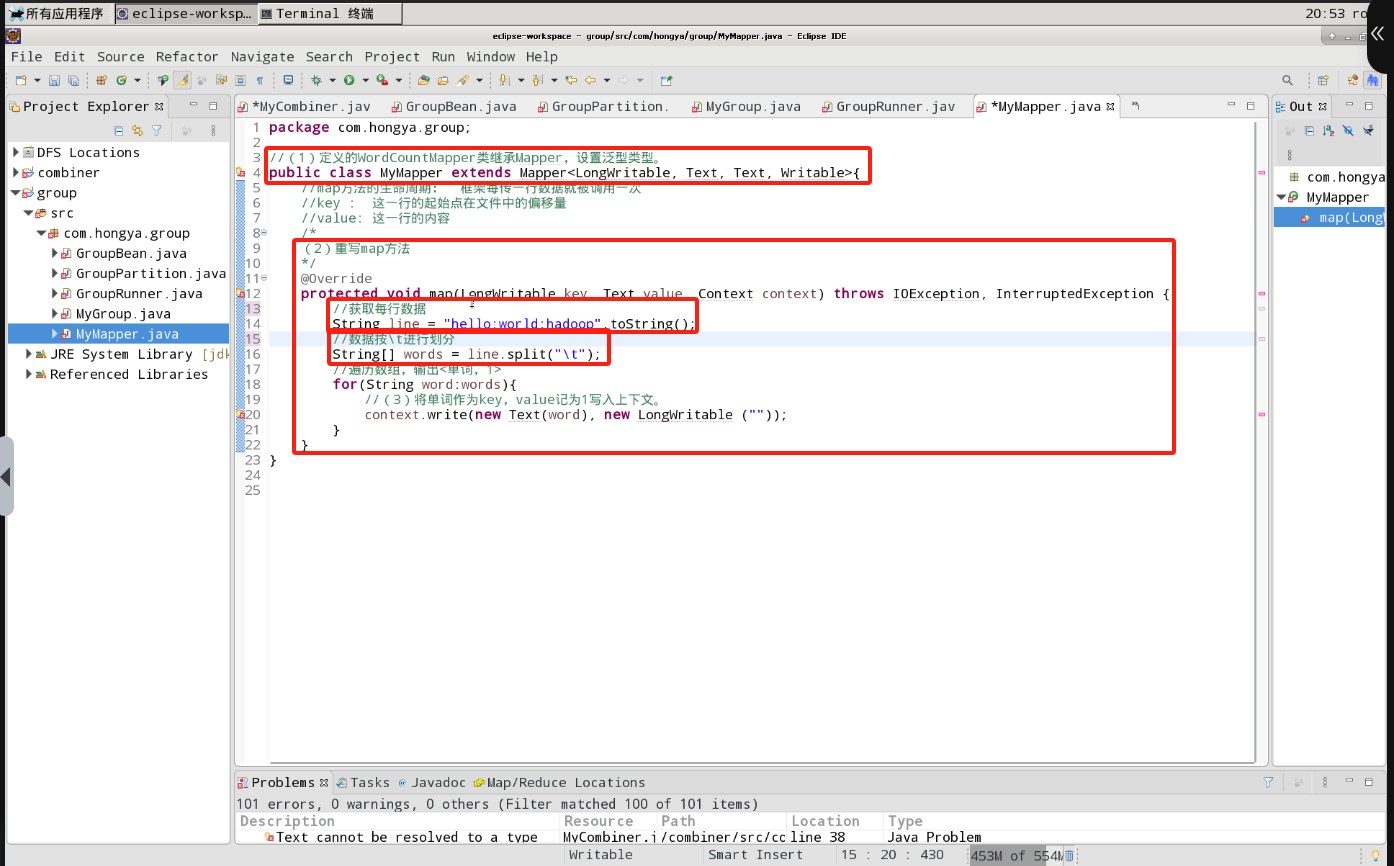
\includegraphics[width=4.5in]{figures/fig25.jpg}
				\end{figure}
			
				Reduce端实现:
				\begin{enumerate}
					\item 定义MyReduce类继承Reducer。
					\item 重写reduce方法。
					\item 收集收据写入上下文。
				\end{enumerate}
				\begin{figure}[H]
					\centering
					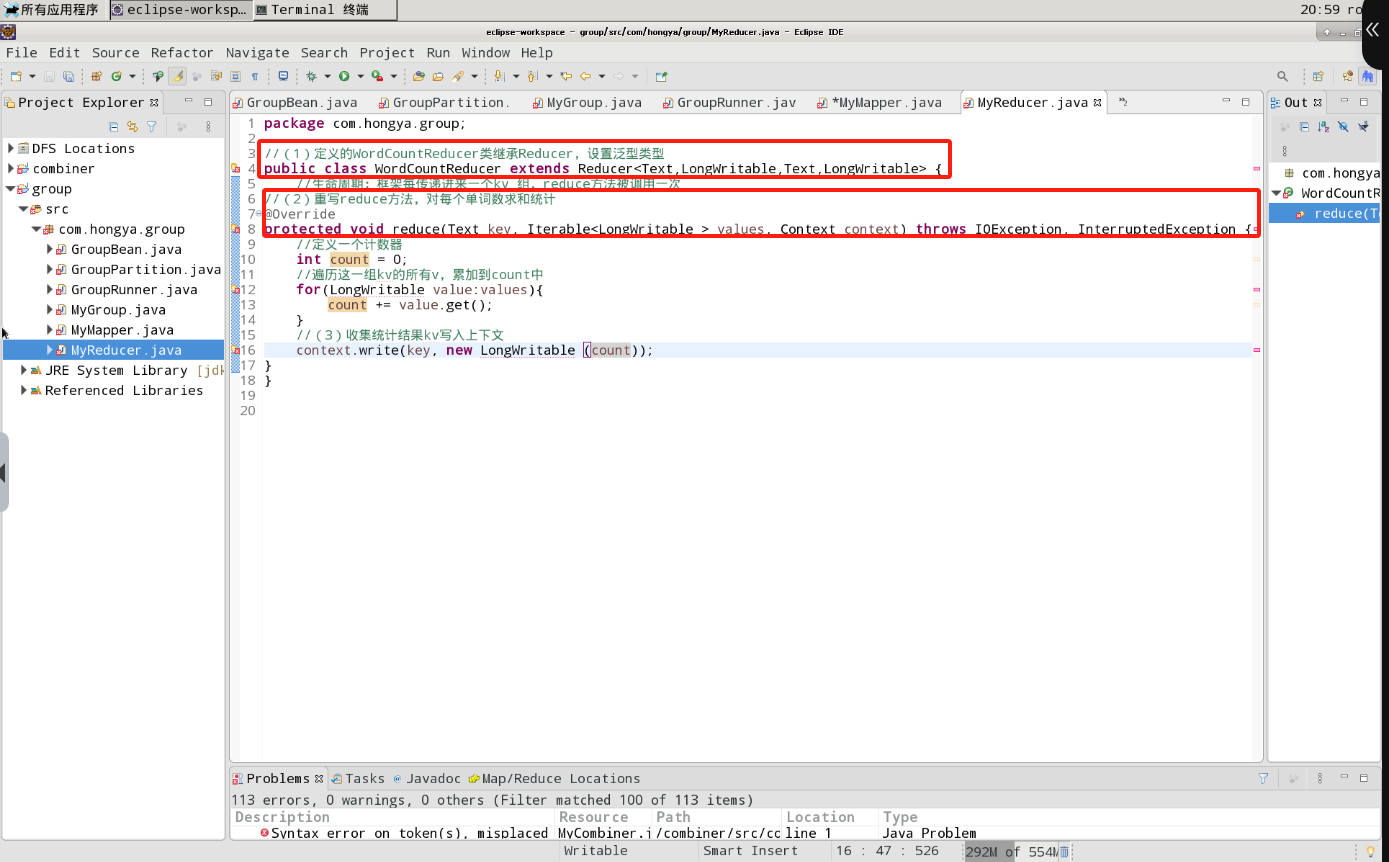
\includegraphics[width=4.5in]{figures/fig26.jpg}
				\end{figure}
			
				运行程序查看结果:
				\begin{enumerate}
					\item 运行程序。
					\item 通过cat 命令查看生成的分区文件part-r-00000,part-r-00001,part-r-00002。
				\end{enumerate}
	
	\section{结果分析}
		MapReducer的Combiner作用是提前分别对Map任务进行分组计数求和,从而节省后续Reduce步骤的计算量和时间,如下图所示:
	
	\section{困难解决}
		7.2、7.3、7.4都碰到了一定的困难。
	
	\section{心得体会}
		做完本次实验,除了掌握了实验目的部分中所有内容的收获之外,我还有以下几点心得体会:
		\begin{itemize}
			\item 掌握了Combiner对于MapReduce过程的作用;
			\item 掌握了MapReduce完整案例的编程。
		\end{itemize}
	
%\end{sloppypar}
\end{document}
\endinput